\chapter{矩阵操作与线性方程组求解}
\begin{introduction}
\item cat、repmat函数
\item 索引与下标
\item find、max、sum函数
\end{introduction}



\section{矩阵生成与性质}
\subsection{矩阵的拼接与复制}
\begin{lstlisting}[frame=single,numbers=left]
% 拼接矩阵
cat(`\mlplaceholder{DIM}`,A,B)
% 举例如下
A=[1 2];
B=[3 4];
% DIM=1,按行拼接
cat(1,A,B) %将得到[1 2 3 4]
% DIM=2,按列拼接
cat(2,A,B) %将得到[1 2;3 4]
\end{lstlisting}

\begin{lstlisting}[frame=single,numbers=left]
% 将矩阵A复制M行N列
repmat(A,`\mlplaceholder{M}`,`\mlplaceholder{N}`)
% 举例如下
A=[1 0];
repmat(A,2,3) % 将得到[1 0 1 0 1 0;1 0 1 0 1 0]
\end{lstlisting}
\subsection{常见工具矩阵}
\begin{lstlisting}[frame=single,numbers=left]
[] %空阵
zeros(n); %n阶全零阵
zeros(m,n); %m行n列全零阵
%ones用法同zeros,全1阵
\end{lstlisting}

\subsection{矩阵基本性质函数}
\begin{lstlisting}[frame=single,numbers=left]
% size函数与length函数
X=zeros(2,3);
D=size(X) %得D=[2,3],行数与列数
L=length(X) %得L=3,相当于max(size(X))
\end{lstlisting}
\section{矩阵操作与分析}
\subsection{索引与下标}
\begin{lstlisting}[frame=single,numbers=left]
% 索引
A(n) %按照(维数>)列>行的顺序标注矩阵元素
% 举例
A=[1,2,3;4,5,6];
A(1:6) %先列后行,结果为 1 4 2 5 3 6
A([end,end-1]) %结果为 6 3
\end{lstlisting}

\begin{lstlisting}[frame=single,numbers=left]
% 下标
A(m,n) %第m行第n列元素
% 举例
A=[1,2,3;4,5,6];
A(2,1) %结果为4
\end{lstlisting}

\begin{lstlisting}[frame=single,numbers=left]
% 排序
sort(A) %第m行第n列元素
% 举例
A=[1,2,3;4,5,6];
A(2,1) %结果为4
\end{lstlisting}

\subsection{逻辑与关系运算与查找}
\begin{lstlisting}[frame=single,numbers=left]
% 查找元素值
A(`\mlplaceholder{condition}`)
% 举例
A=[1,2,3;4,5,6];
A(A-2==0|A-3==0|A-4==0) %按列查找,结果为[4;2;3]
\end{lstlisting}

\begin{lstlisting}[frame=single,numbers=left]
% 查找元素索引
find(`\mlplaceholder{condition}`)
% 举例
A=[1,2,3;4,5,6];
find(A-2==0|A-3==0|A-4==0) %按列查找,结果为[2;3;5]
\end{lstlisting}

\begin{lstlisting}[frame=single,numbers=left]
% 查找元素最大值
max(A)
% 举例
A=[1,2,3;4,5,6];
max(A) %每列最大值,结果为[4 5 6]
[Rmax I]=max(A) %Rmax=[4 5 6],I=[2;2;2],返回在指定维度中的位置
\end{lstlisting}
\subsection{矩阵分析}
\begin{lstlisting}[frame=single,numbers=left]
% 求和
sum(A)
% 举例
A=[1,2,3;4,5,6];
sum(A) %按列求和,结果为[5 7 9]
sum(A,2) %按行求和,结果为[6;15]
\end{lstlisting}

\section{线性方程组的求解}
\subsection{高斯消元法}
\begin{definition}{高斯消元法}{}
基本思路为:化为上三角阵,回代求解。
\end{definition}

对于方程组
\[
AX=\emph{\textbf{b}}
\]

解可以表示为
\[
X=A\_\emph{\textbf{b}}
\]
\subsection{作答模板}
\begin{lstlisting}[frame=single,numbers=left]
% 得到所需矩阵A、b,注意对齐方式!
A=[`\mlplaceholder{系数矩阵}`];b=[`\mlplaceholder{增广矩阵}`];
% 使用左除命令求解
x=A\b;
\end{lstlisting}
\begin{problem}
假设一混合物由硝基苯$C_6H_5NO_2$、苯胺$C_6H_7N$、氨基丙酮$C_3H_7NO$和乙醇$C_2H_6O$组成。对该混合物进行元素分析,结果各元素\footnote{原子量:C为12,H为1,0为16,N为14。}的质量百分数为:$w_C=\SI{57.78}{\percent},w_H= \SI{7.92}{\percent},w_N= \SI{11.23}{\percent},w_O= \SI{23.07}{\percent}$。试编写一个MATLAB函数:

1)确定上面四种化合物在混合物中所占的质量百分数,采用 fprintf 函数将结果显示在屏幕上;

2) 检验求得的质量分数之和是否为 1,如果是则在屏幕上显示信息:Calculation succeed。如果否,则显示警告信息:The calculation is wrong。
\end{problem}

\begin{solution}
\begin{lstlisting}
function example2_1
N=[6 5 1 2;6 7 1 0;3 7 1 1;2 6 0 1]; %四种分子中的C、H、N、O数,顺序下同
M=[12 1 14 16];% 原子量
M=repmat(M,4,1);
A=M.*N; % 原子量之和
% 分子中,四种元素的质量分数
A(1,:)=A(1,:)/sum(A(1,:));
A(2,:)=A(2,:)/sum(A(2,:));
A(3,:)=A(3,:)/sum(A(3,:));
A(4,:)=A(4,:)/sum(A(4,:));
b=[0.5778 0.0792 0.1123 0.2307]';% 总质量分数
x=A'\b;% 关键命令!
% 两位精度显示,并自动换行
fprintf('The percentage of C6H5NO2 is %.2f%%\n',100*x(1))
fprintf('The percentage of C6H7N is %.2f%%\n',100*x(2))
fprintf('The percentage of C3H7NO is %.2f%%\n',100*x(3))
fprintf('The percentage of C2H6O is %.2f%%\n',100*x(4))
if sum(x)==1
    disp('Calculation succed')
else
    warning('The calculation is wrong')
end
\end{lstlisting}

\begin{figure}[htbp]
\centering
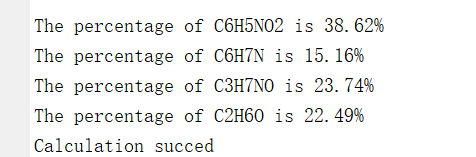
\includegraphics[width=0.5\textwidth]{exampe2_1.png}
\caption{运行结果}
\end{figure}

\end{solution}